\documentclass[twocolumn,10pt,cleanfoot]{asme2ej}

\usepackage[utf8]{inputenc}
\usepackage[
  main=czech,
  czech, english
]{babel}
\usepackage{epsfig} %% for loading postscript figures


\usepackage[backend=biber, 		% use biber as backend instead of BiBTeX
	citestyle=numeric, 		    % citation style
	url=true, 			        % display urls in bibliography
	hyperref=auto,			    % detect hyperref and create links
]{biblatex}
\addbibresource{report.bib}
\usepackage{url}
\usepackage{hyperref}


\title{IV109 Modelování a simulace:\\Zpětné vazby v adaptabilních systémech}

\author{
    \textmd{Jan Horáček}
    \affiliation{
    445326@mail.muni.cz
    }
    \and
    Tomáš Effenberger
    \affiliation{
    410350@mail.muni.cz
    }

}

%\author{Tomáš Effenberger
%    \affiliation{
%    410350@mail.muni.cz
%    }
%}



\begin{document}

\maketitle

%%%%%%%%%%%%%%%%%%%%%%%%%%%%%%%%%%%%%%%%%%%%%%%%%%%%%%%%%%%%%%%%%%%%%%
\section{Téma}

Nástup internetu a moderních počítačových technologií již delší dobu neznamená pouze ulehčení komunikace, ale také možnost, jak se efektivně učit. Výuku ve školních lavicích doplňují hodiny strávené na webových stránkách, které dětem více či méně efektivně poskytují přísun znalostí, po kterých tak touží.


Je odpovědností informatiků, aby pozorování YouTube videí bylo nahrazeno efektivními vyučovacími metody. Aby bylo učení co možná nejefektivnější, je žádoucí výukový systém nastavit na míru konkrétnímu studentovi, například dát každému studentovi jiný počet otázek v závislosti na jeho odpovědích (resp. výkonech). Navíc je vhodné, aby se systém samotný za základě posbíraných dat učil (například které otázky jsou pro studenty nejvhodnější, nejlehčí, nejtěžší, atp.). Byla by škoda nevyužít současných prostředků, které umožňují ve velkém sbírat data o studentech a na základě jejich chování upravovat chování systému.

Systémům, které takto fungují, se říká adaptabilní.
Takový systém si můžeme představit jako webovou stránku, která dává uživatelům úlohy např. různých náročností podle toho, jak odhaduje schopnosti studenta. Adaptabilní systém se snaží dát studentovi otázku, ze které se (například) nejvíc naučí, ale zároveň otázku, která není nad jeho síly.

%%%%%%%%%%%%%%%%%%%%%%%%%%%%%%%%%%%%%%%%%%%%%%%%%%%%%%%%%%%%%%%%%%%%%%
\section{Problém}

Tento projekt se zaměřuje na analýzu adaptabilních výukových systémů s důrazem na hledání anomálií, které mohou vést k postupné degradaci chování systému. Takovouto degradaci si můžeme představit třeba tak, že systém, který průběžně rozhoduje, kdy jím student úspěšně prošel, po několika týdnech posune pomyslnou laťku pro úspěšné projití nesmyslně vysoko nebo naopak nesmyslně nízko.

V tomto projektu zkoumáme, zda existují takové parametry prostředí, které mohou vést k tomu, že výukový systém nastaví hranici \emph{úspěšného projití systémem} (resp. naučení se tématu) příliš vysoko, či příliš nízko.

%\newpage

%%%%%%%%%%%%%%%%%%%%%%%%%%%%%%%%%%%%%%%%%%%%%%%%%%%%%%%%%%%%%%%%%%%%%%
\section{Model}

Náš model obsahuje adaptabilní výukový systém a studenty, kteří se v tomto systému učí. Systém procvičuje jediný koncept a využívá \emph{mastery learning} -- předkládá studentům úlohy, dokud neuzná, že už student koncept umí. Všechny úlohy mají stejnou obtížnost.

% \subsection{Model studenta}
Dovednost studentů modelujeme pomocí \emph{BKT}, tj. student buď procvičovaný koncept umí nebo neumí a po každé úloze má konstantní pravděpodobnost naučení se. To, zda koncept umí nebo neumí, ovlivňuje pravděpodobnost podání slabého nebo silného výkonu. Silný výkon interpretujeme jako rychlé a bezchybné vyřešení zadaného úkolu. Modelujeme nehomogenní populaci: existuje několik typů studentů; pro každý typ jsme použili některou čtveřici parametrů detekovanou jako “běžnou” při analýze systému na výuku matematiky v článku \cite{bkt-reduce}. Kromě dovednosti modelujeme ještě trpělivost studenta, tj. kolik silných výkonů v řadě může provést, než ho procvičování přestane bavit a odejde (protože koncept už umí).

% \subsection{Model systému}
Modelovaný výukový systém potřebuje odhadovat aktuální dovednost studenta, tj. musí sám obsahovat model studenta (podobně jako v \cite{bkt-optimal-worst}). Model studenta uvnitř systému nazýváme \emph{proxy student} (a studenta vně systému nazýváme jako \emph{skutečný student}). Systém modeluje pouze dovednost studentů, nikoliv trpělivost. Na druhou stranu je modelovaný scénář optimistický v tom, že struktura modelu dovedností proxy studenta přesně odpovídá struktuře modelu skutečného studenta. Systém nezná jednotlivé podpopulace studentů, takže pro BKT využívá průměrné hodnoty parametrů. Pro analýzy pak přidáváme ještě parametr udávající šum v odhadu parametrů (konstantní posun ve všech parametrech oproti průměru v populaci).

Systém dále obsahuje hranici pro mastery -- pokud pravděpodobnost znalosti konceptu přesáhne tuto hranici, systém deklaruje mastery a student úspěšně prošel. Tuto hranici se systém snaží v dlouhodobém horizontu (týdny) optimalizovat pomocí série AB experimentů. V každém týdnu do systému přijde N nových studentů, systém je rozdělí do dvou skupin a pro každou z nich používá jinou hranici pro mastery (aktuální hranice $\pm$ malý posun). Každému studentovi dává úlohy tak dlouho, dokud buď chce řešit, nebo dokud systém nedeklaruje mastery. Po zpracování všech N studentů systém použije metriku pro vyhodnocení kvality systému při těchto dvou hranicích a posune aktuální hranici směrem k~lepší z~těchto dvou možností.

V analýzách uvedených v této zprávě používáme následující metriku: rozdíl počtu úloh se slabým a silným výkonem. (Slabý výkon odpovídá tomu, že se student učí, takže počet těchto pokusů chceme maximalizovat, zatímco silný výkon znamená, že už to nejspíš umí a nudí se, což chceme naopak minimalizovat.) Systém provádí mnoho iterací takovýchto AB experimentů (vždy na nových studentech) ve snaze postupně vylepšovat chování systému změnou hranice pro mastery.

%%%%%%%%%%%%%%%% begin figure %%%%%%%%%%%%%%%%%%%
\begin{figure}[htb]
\centering
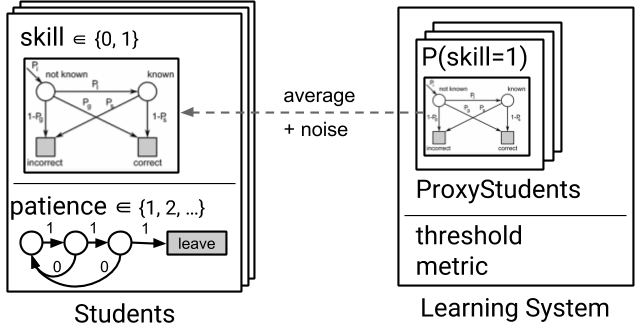
\includegraphics[width=\columnwidth]{img/model}
\caption{Schéma použitého modelu adaptabilního výukového systému a studentů.
  Obrázek BKT převzatý z \cite{bkt-logistic-overview}.}
\label{fig:model}
\end{figure}
%%%%%%%%%%%%%%%% end figure %%%%%%%%%%%%%%%%%%%

% \subsection{Zpětné vazby}
Aktuální hranice pro mastery ovlivňuje posbíraná data (pokud je hranice vyšší, studenti procvičují déle), posbíraná data ovlivňují vyhodnocení, výsledek vyhodnocení ovlivňuje hranici. Jak uvidíme později, tato vazba může být pozitivní a hnát tak hranici do extrému. Situaci, kdy hranice degeneruje k 1 (a zůstane tam) nazýváme anomálií a sledujeme, jak často k ní dochází (průměr přes mnoho běhů celé simulace).

%%%%%%%%%%%%%%%%%%%%%%%%%%%%%%%%%%%%%%%%%%%%%%%%%%%%%%%%%%%%%%%%%%%%%%
\section{Simulace}

Základním prvkem simulace jsou modely studenta, v~našem případě \emph{proxy student} a
\emph{skutečný student}. Nyní prakticky demonstrujeme rozdíly v chování těchto dvou modelů v naší simulaci.
Obrázek \ref{fig:bkt} zobrazuje dovednost skutečného studenta (zelená křivka) srovnanou s dovedností proxy studenta (modrá křivka). Graf navíc uvádí odpovědi studenta na otázku (červené body), kde 0 je slabý výkon a 1 je silný výkon.


%%%%%%%%%%%%%%%% begin figure %%%%%%%%%%%%%%%%%%%
\begin{figure}[htb]
\centering
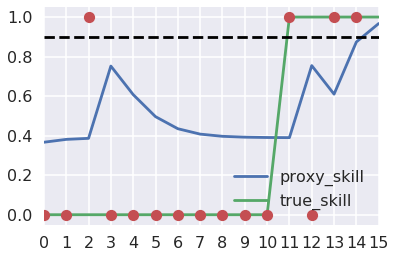
\includegraphics[width=\columnwidth]{img/bkt}
\caption{BKT}
\label{fig:bkt}
\end{figure}
%%%%%%%%%%%%%%%% end figure %%%%%%%%%%%%%%%%%%%

Z grafu je patrné, že proxy dovednost je skutečně aproximací skutečné dovednosti studenta. Je také vidět, že pokud student podá silný výkon, výukový systém výrazně zvýší odhad jeho schopností, zatímco po slabém výkonu se odhad schopností zvýší jen nepatrně, nebo dokonce sníží. Graf dále zobrazuje dovednost, která je nutná pro deklarování mastery (černá přerušovaná úsečka). Z grafu je patrné, že studentovi bylo deklarováno mastery až čtyři otázky poté, co se student koncept naučil.

Zkoumali jsme chování systému pro základní proxy metriky. Obrázek \ref{fig:thresholds-solved-tasks} ukazuje vývoj hranice pro mastery v čase při optimalizaci proxy metriky \emph{počtu vyřešených úloh}.
Na tomto výsledku ilustrujeme především to, že náš model se chová logicky. Výukový systém se snaží dosáhnout co největšího počtu vyřešených úloh. Jeho cestou k tomuto cíli je posunout laťku úspěšnosti na maximum, takže studenti zůstanou ve výukovém systému dlouho a vyřeší co nejvíce úloh. Toto chování označujeme za \emph{degenerované}, avšak dodáváme, že se nejedná o něco, na co bychom potřebovali složitou simulaci. Na zjištění tohoto důsledku by stačil selský rozum.

%%%%%%%%%%%%%%%% begin figure %%%%%%%%%%%%%%%%%%%
\begin{figure}[htb]
\centering
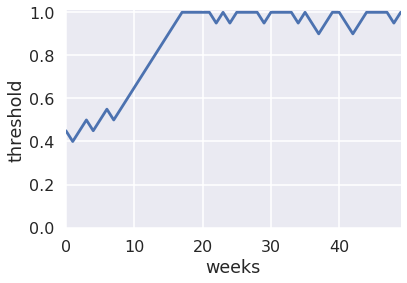
\includegraphics[width=\columnwidth]{img/thresholds-solved-tasks}
\caption{Vývoj hranice pro mastery při optimalizaci metriky počtu všech vyřešených úloh.}
\label{fig:thresholds-solved-tasks}
\end{figure}
%%%%%%%%%%%%%%%% end figure %%%%%%%%%%%%%%%%%%%


Proto jsme přistoupili k simulaci dalších proxy metrik. Vyzkoušeli jsme maximalizovat počet úspěšně vyřešených úloh, což dopadlo stejně, jako v předchozí metrice. Dále jsme vyzkoušeli cílit na proxy dovednost rovnou konkrétnímu číslu (např. 0.85). Výsledek je vyobrazen na obrázku \ref{fig:thresholds-target-skill}.
Tato metrika už se chovala poměrně hezky a k anomáliím nedocházelo. Avšak opět se jedná o poměrně logický důsledek.

%%%%%%%%%%%%%%%% begin figure %%%%%%%%%%%%%%%%%%%
\begin{figure}[htb]
\centering
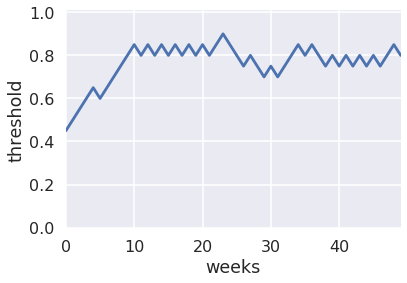
\includegraphics[width=\columnwidth]{img/thresholds-target-skill}
\caption{Vývoj hranice pro mastery při optimalizaci metriky vzdálenosti od cílové dovednosti.}
\label{fig:thresholds-target-skill}
\end{figure}
%%%%%%%%%%%%%%%% end figure %%%%%%%%%%%%%%%%%%%


Pro následující analýzy jsme nakonec použili proxy metriku, která se snaží maximalizovat rozdíl efektivních (student se něco naučil) a neefektivních otázek (student se nic nenaučil).
U této metriky už není tak zřejmé, jak by se měl chovat. Při základních parametrech, kdy neprovádíme umělé zašumění dat, se metrika chová rozumně
(Obrázek \ref{fig:thresholds-effective-tasks}).
Začali jsme tedy zkoumat, jak se metrika chová, pokud výukový systém nemá o studentech úplná data.

%%%%%%%%%%%%%%%% begin figure %%%%%%%%%%%%%%%%%%%
\begin{figure}[htb]
\centering
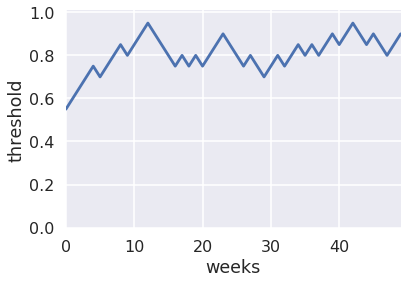
\includegraphics[width=\columnwidth]{img/thresholds-effective-tasks}
\caption{Vývoj hranice pro mastery při optimalizaci metriky počtu efektivních otázek.}
\label{fig:thresholds-effective-tasks}
\end{figure}
%%%%%%%%%%%%%%%% end figure %%%%%%%%%%%%%%%%%%%

%%%%%%%%%%%%%%%%%%%%%%%%%%%%%%%%%%%%%%%%%%%%%%%%%%%%%%%%%%%%%%%%%%%%%%
\section{Analýzy}

Zkoumali jsme, jak často dochází k anomáliím v~závislosti na (1) šumu v modelu dovedností (nepřesnost parametrů BKT), (2) netrpělivosti skutečných studentů a (3) počtu studentů v systému. Pokud je trpělivost studentů nekonečná (nebo dostatečně vysoká), pak k anomáliím vůbec nedochází (nezávisle na šumu). Podobně, pokud jsou BKT parametry přesné (šum 0) a netrpělivost není úplně extrémní (alespoň 3), tak k anomáliím také nedochází. Pokud však je v odhadu parametrů šum a současně jsou studenti netrpěliví, pak k anomáliím dochází.

Pro danou netrpělivost míra anomálií roste se zvyšujícím se šumem.
Obrázek \ref{fig:anomaly-noise} ukazuje frekvenci v~závislosti na míře šumu, při fixní netrpělivosti.
Podobně roste míra anomálií se zvyšující se netrpělivostí studentů.
(Obrázek \ref{fig:anomaly-patience}).
Nakonec jsme ověřili, že frekvence anomálií nezávisí na počtu studentů v~systému
(Obrázek (\ref{fig:anomaly-students}).

%%%%%%%%%%%%%%%% begin figure %%%%%%%%%%%%%%%%%%%
\begin{figure}[htb]
\centering
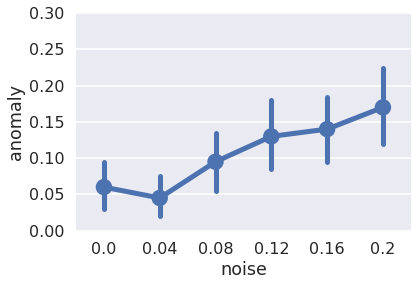
\includegraphics[width=\columnwidth]{img/anomaly-noise}
\caption{Závislost frekvence anomálií (jak často došlo k anomáliím, zprůměrováno přes 200 běhů) v závislosti na míře šumu, při 100 studentech v systému, kteří mají všichni trpělivost 3. Vertikální čáry znázorňují 95\% intervaly spolehlivosti spočítané pomocí bootstrappingu.}
\label{fig:anomaly-noise}
\end{figure}
%%%%%%%%%%%%%%%% end figure %%%%%%%%%%%%%%%%%%%


%%%%%%%%%%%%%%%% begin figure %%%%%%%%%%%%%%%%%%%
\begin{figure}[htb]
\centering
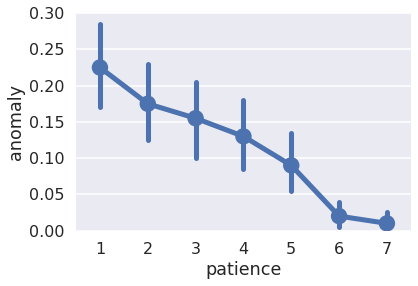
\includegraphics[width=\columnwidth]{img/anomaly-patience}
\caption{%
  Závislost frekvence anomálií na trpělivosti studentů.
  Simulace se 100 studenty v systému a šumu v parametrech 0.2.}
\label{fig:anomaly-patience}
\end{figure}
%%%%%%%%%%%%%%%% end figure %%%%%%%%%%%%%%%%%%%


%%%%%%%%%%%%%%%% begin figure %%%%%%%%%%%%%%%%%%%
\begin{figure}[htb]
\centering
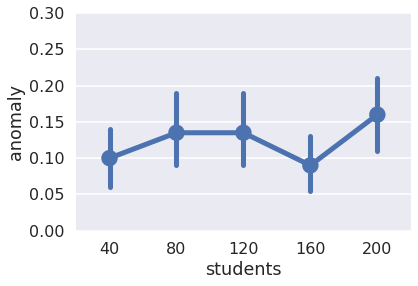
\includegraphics[width=\columnwidth]{img/anomaly-students}
\caption{%
  Závislost frekvence anomálií na počtu studentů,
  při trpělivosti 3 a šumu v BKT parametrech 0.2.}
\label{fig:anomaly-students}
\end{figure}
%%%%%%%%%%%%%%%% end figure %%%%%%%%%%%%%%%%%%%


%%%%%%%%%%%%%%%%%%%%%%%%%%%%%%%%%%%%%%%%%%%%%%%%%%%%%%%%%%%%%%%%%%%%%%
\section{Závěr}

Simulace ukazuje, jak v adaptabilním výukovém systému, který se iterativně vylepšuje na základě výsledků AB experimentů podle nějaké zdánlivě rozumné proxy metriky, může nepřesnost používaného modelu studenta vést k~anomálii, kdy se hranice pro mastery postupně vysune až na 1 (tj. systém nikdy nenechá studenta projít). V našem scénáři spočívala nepřesnost jednak v zanedbání trpělivosti studentů a jednak v zašuměných parametrech modelu dovednosti.

Je však možné, že anomálie není způsobena vyhodnocováním na ovlivněných datech, ale pouze “self-selection biasem” (studenti si sami regulují procvičování díky své netrpělivosti) a docházelo by k ní i při vyhodnocení, které by bylo férové vzhledem k vyhodnocovaným hranicím (vyhodnocovalo by je na stejných datech). Bylo by proto možná vhodnější sledovat i nějakou metriku počítanou nad skutečnými studenty a definovat anomálii jako snižování této metriky (při současném zvyšování proxy metriky). Pokud by se i tato “skutečná” metrika zvyšovala, pak není problém ve vyhodnocování na různě posbíraných datech. K lepšímu pochopení problému bychom ideálně chtěli najít co nejjednodušší scénář, ve kterém bude docházet k anomálii a přitom nebude obsahovat self-selection bias.

Jako další krok se pak nabízí zkoumání strategií zásahů k redukci anomálie pomocí férovějšího vyhodnocení, např. použitím důmyslnějších metrik, nebo multiobjektivní optimalizací, kdy by systém sledoval více různých metrik a posunul hranici pouze při zlepšení ve všech sledovaných metrikách. Jiná strategie je nechat některé studenty procvičovat o~něco déle, než do momentu dosažení mastery podle systémů, a umožnit tak vyhodnocení různých hranic na stejných datech. Ještě zajímavější strategie se pak nabízí v případě systému s více levely, kdy si můžeme dovolit studenta pustit do dalšího levelu hned, když si myslíme, že už úlohy v~tomto levelu zvládá, a až později si pomocí občasné náhodně zvolené úlohy z nižšího levelu ověřit, že tyto levely opravdu zvládl.


\printbibliography[heading=bibintoc]

\end{document}
